\begin{figure}
  \caption{Income distributions by treatment group and census year} \centering
  \label{fig:group-incwage-dist}
  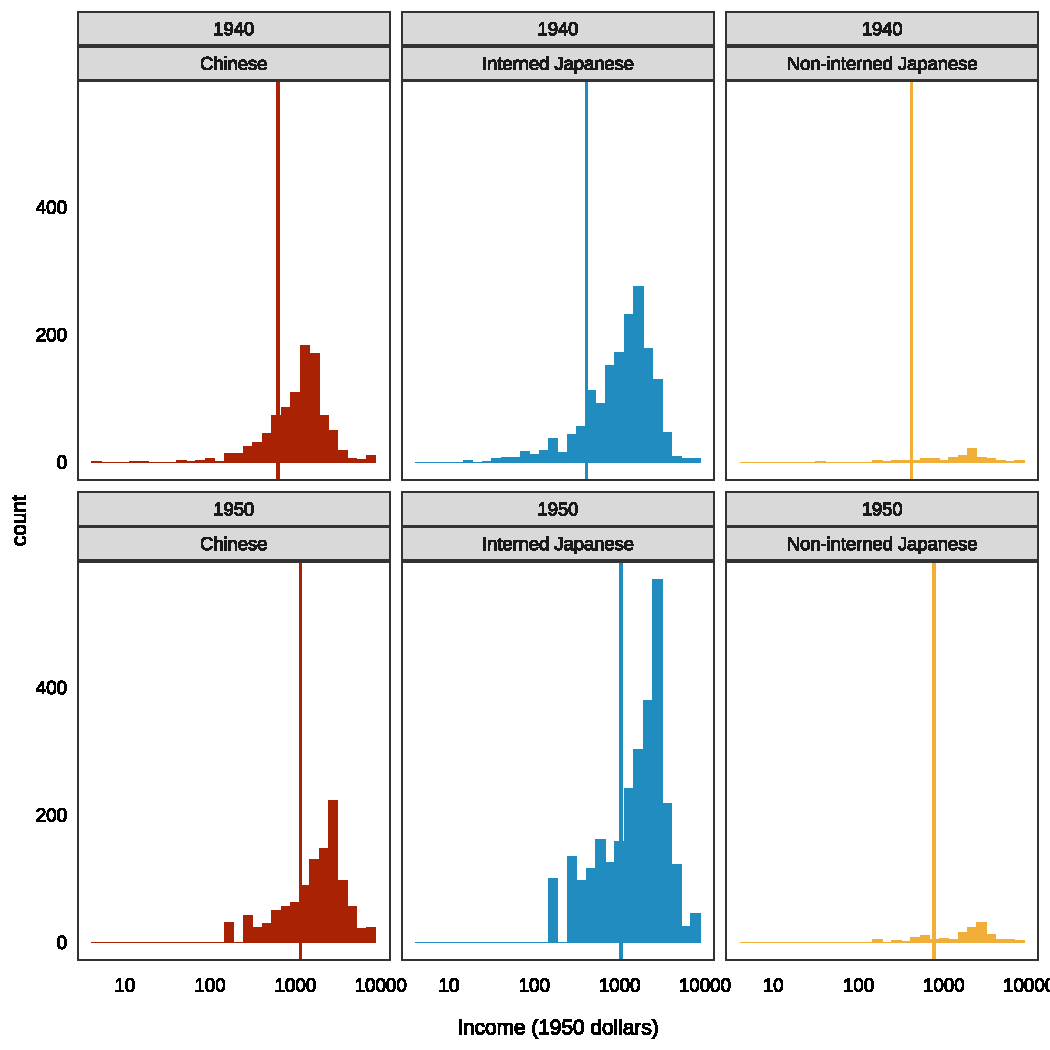
\includegraphics[width=\textwidth]{../figures/group-incwage-dist.pdf} \\
  \caption*{
    \footnotesize
    \emph{Note:}
    These histograms include all linked individuals
    from the main analysis sample.
    All Chinese individuals are treated as non-interned.
    `Interned Japanese' include all Japanese individuals
    with an estimated probability of greater than 0.75.
    `Non-interned Japanese' include all Japanese
    with an estimated probability equal to zero.
    Japanese with a probability between 0 and 0.75 are omitted
    in this figure.
    INCWAGE is the total earnings through wage employment
    from the year prior to each census year.
    Incomes in 1940 are adjusted for inflation to 1950 dollar amounts.
    }
\end{figure}